\documentclass[12pt,a4paper]{Cotmas-2018}

\usepackage[czech]{babel}
\usepackage{csquotes}
\usepackage{graphicx}
\usepackage{textcomp}
\usepackage{caption}
\usepackage{biblatex}
\addbibresource{bibliography.bib}

% rovnice zarovnávat doleva
\usepackage[fleqn]{amsmath}

% neodsazovat nové odstavce
\setlength{\parindent}{0pt}


\begin{document}

%%%%%%%%%%%%%%%% TITLE PAGE %%%%%%%%%%%%%%%%
\begin{titlepage}
\begin{center}

\includegraphics[width=0.5\linewidth]{img/logo.pdf}
\vspace{3cm}

\LARGE\uppercase{Modelování a simulace 2021/2022}
\vspace{1cm}

\LARGE\textbf{Simulační studie na technologii Vehicle-to-grid}

\vspace*{\fill}
\large{Ondřej Mach (xmacho12)}

\large{Rostislav Lán (xlanro00)}

\end{center}
\end{titlepage}


%%%%%%%%%%%%%%%% TABLE OF CONTENTS %%%%%%%%%%%%%%%%
\pagenumbering{arabic}
\setcounter{page}{1}
\tableofcontents
\clearpage

%%%%%%%%%%%%%%%% THE ACTUAL DOCUMENT %%%%%%%%%%%%%%%%

\section{Úvod}
Tato práce pokládá otázku, zda je technologie Vehicle-to-grid ekonomicky rentabilní.
Přínos této technologie je posouzen podle simulačního modelu, který modeluje výrobu a spotřebu elektrické energie v rámci domu.
Technologie je poměrně nová a studie na toto téma dochází k různým závěrům, což bylo motivací pro vytvoření tohoto projektu.

\subsection{Technologie Vehicle-to-grid}
Vehicle to Grid (dále jen V2G) je technologie využívající vozidla schopná uchovávat nebo vyrábět(např. některé typy vodíkových vozidel) elektrickou energii. V2G umožňuje nečinným vozidlům zapojeným do sítě využívat v nich uloženou elektrickou energii  za účelem napájení části nebo celé domácnosti anebo dodávat tuto energii do sítě.
Vyžaduje datové spojení mezi vozidlem a nabíjecí stanicí, umožňující monitorovat stav sítě a podle napětí v síti modifikovat množství nabíjené elektřiny.

\subsection{Motivace vzniku a výhody Vehicle-to-grid}
Primárních cílů technologie V2G je několik.

Za prvé jsou baterie elektrických vozidel prostředkem pro vybalancování stavu sítě. Toho je zapotřebí zejména v případě, že energie v síti pochází z významné části z obnovitelných zdrojů. Ty jsou totiž volatilní, tedy, že při růžných podmínkách mohou produkovat značně rozdílné množství energie. To může způsobit snížení napětí při nedostatečné produkci, přetížení sítě v dané oblasti při příliš nadměrné produkci elektřiny, nebo zacpání sítě. Toto pak způsobuje prodražení kupované elektřiny, protože se začne odebírat ze záložních tedy i dražších elektráren. Technologie V2G dokáže při dostatečně rozsáhlém zavedení zmenšit následky, nebo úplně zamezit některým z těchto jevů 
\cite{Greaker-Hagem-Proost-2022}.

Pro zákazníka to tedy znamená, že mu V2G systém umožňuje nabíjet baterii v časy, kdy je elektřina levnější a napopak ji při vysokých cenách dodávat do sítě nazpět, nebo alespoň z části pokrýt spotřebu domácnosti. Tím může zákazníkovi výrazně snížit výdaje za elektřinu 
\cite{Virta-Ltd-2021}.

\subsection{Nevýhody Vehicle-to-grid}
V rámci procesu nabíjení a dodávání elektřiny do a ze sítě však dochází, stejně jako při jízdě a nabíjení, k opotřebení baterie, tudíž ke snížení životnosti vozidla. Vzhledem k vysokému podílu ceny baterií na ceně elektrického vozidla to nemusí být ekonomicky výhodné.
Dále je spekulovatelná škálovatelnost, z důvodů kompatibility vozidel při zapojení do sítě 
\cite{Lakshmi-Divya-Sravani-2019}.

\subsection{Konfigurace zapojení elektrických vozidel}
Systém V2G může být nakonfigurován více způsoby.
V1G, neboli jednosměrné V2G, je režim, kdy vozidlo nemůže dodávat do sítě elektřinu,
je však schopno určit nejvhodnější časy pro nabíjení ze sítě. To mu umožňuje významně snížit cenu nabíjení, zátěž sítě a využívat větší podíl elektřiny z obnovitelných zdrojů.
V2B/V2H, neboli vehicle-to-building/home, při tomto režimu je vozidlo schopné omezeně dodávat uloženou energii do budovy/domácnosti v případě fluktuace napští v síti, nebo při výpadcích proudu.
V2X, jinak také vehicle-to-everything, režim zamšřený na komunikaci s ostatními vozidly nebo infrastrukturou, primárním účelem není kontrola nabíjení, ale efektivita a bezpečnost dopravy.
V2G - vehicle-to-grid, nebo bi-directional smart charging. Umožňuje dodávat vyráběnou/uchovávanou elektřinu zpět do sítě a tím snížit její zatížení 
\cite{Svarc-2022}.

\subsection{Předchozí studie}
Tímto tématem se již v minulosti zabývalo množství odborných studií. Jejich cílem bylo zjistit použitelnost konceptu a zjistit jeho benefity a nevýhody. 

Bylo zjištěno, že pravidelným nabíjením a vybíjením baterie při provozu vozidla jako V2G dochází k degradaci baterie elektrického vozidla a tím ke snížení její životnosti 
\cite{Shirazi-2018}.
Dopady na baterii však lze zmírnit použitím inteligentních sítí 
\cite{University-of-Warwick-2017}.

\section{Simulační model}
Simulační model je logicky rozdělen na domácnost, solární elektrárnu, elektrické vozidlo a měřící zařízení.

\bigskip
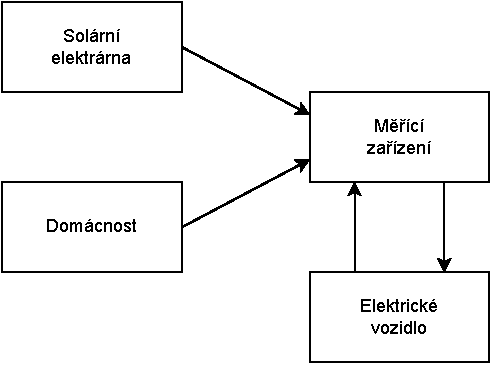
\includegraphics[width=0.5\linewidth]{img/diagram.pdf}
\bigskip

V rámci solární elektrárny je náhodně generován výkon.
Ten je závislý pouze na modelovém čase, ze kterého je určeno roční období.

Modul domácnosti generuje spotřebovaný výkon, který je také závislý na čase,

\subsection{Solární elektrárna}
V rámci tohoto modulu je náhodně generována výroba energie.
Jediným výstupem je tudíž proměnná, ve které je uložen výkon elektrárny v daném čase.
Vstupem pro toto generování je čas, podle kterého je určeno roční období.
To má v realitě významný vliv na výkon elektrárny, proto je nutné ho brát v úvahu.

Konkrétními faktory, které mají významný vliv na výrobu elektřiny jsou délka dne, pozice slunce na obloze, natočení panelu na světovou stranu, úhel panelu vzhledem k zemi a počasí. Znečištění ani poškození panelu není bráno v úvahu.

Délka dne je určována z dat o východu a západu slunce, panel je uvažován napevno přidělaný pod konstantním úhlem 45°.
Pozice slunce je určena tabulkou, ve které jsou vypsány průměrné hodnoty efektivity panelů v daných ročních obdobích(nezávislé na počasí - tzn. v tabulce jsou slunečné dny). Tyto hodnoty se vztahují k Německu, avšak vzhledem k velmi podobným geografickým a meterologickým podmínkám byly použity pro nedostatek lokálnějšího zdroje 
\cite{German-solar-hourly-2014}.

 Měnící se efektivita je viditelná na grafu~\ref{fig:solar_month}, kde je během měsíce dubna dobře viditelný rostoucí výkon elektrárny v jasných dnech. Zároveň je patrný rozdíl slunečnými a oblačnými dny \cite{PF-Bach-2022}.

\begin{figure}
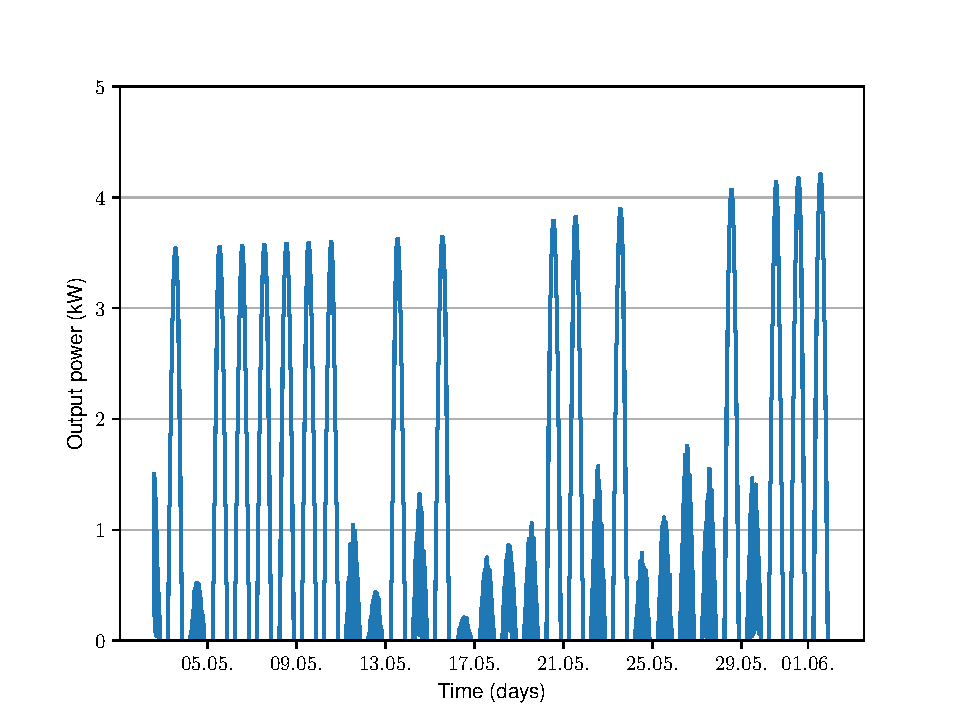
\includegraphics[width=\linewidth]{img/solar_month.pdf}
\caption{Výkon solárního panelu během dubna}
\label{fig:solar_month}
\end{figure}

Protože se efektivita panelu snižuje při vyšších teplotách vzduchu, jsou hodnoty v každém měsíci přepočítány pro průměrné teploty daného měsíce pomocí tabulky s hodnotami teploty během roku, což v případě České republiky vede ke snížení celkového výkonu elektrárny \cite{Cotmas-2018}.

Započítáno je zde i pro kratší období zanedbatelné půlprocentní opotřebení panelu za rok, které se významně projeví pouze při simulacích několika let.

Počasí je simulováno dle počtu hodin, kdy během měsíce svítí slunce. Ten se vydělí délkou daného dne a takto získáme počet slunečných dní. Změna výkonu  v závislosti na čase během slunečného dne se nachází na grafu~\ref{fig:solar_day_clear} \cite{Journal-of-PV-2020}.

\begin{figure}
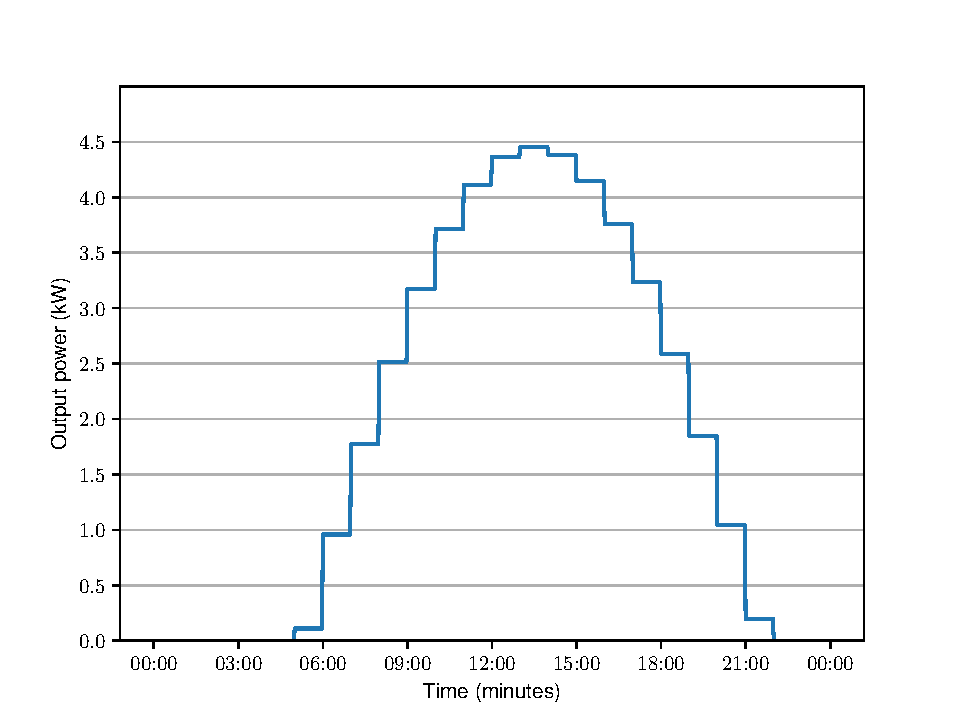
\includegraphics[width=\linewidth]{img/solar_day_clear.pdf}
\caption{Výkon solárního panelu během jasného letního dne}
\label{fig:solar_day_clear}
\end{figure}

Zatažené dny jsou v měsíci vybírány náhodně tak, aby celkový počet slunečných a zatažených hodin v měsíci se rovnal sumě počtu hodin mezi východem a západem slunce. Intenzita zataženosti je počítána jako průměr předchozí hodnoty zataženosti a hodnoty náhodné. Tímto způsebem získáme hodnoty, které odpovídají hodnotám skutečně naměřeným. Výkon elektrárny během oblačného dne se nachází v grafu~\ref{fig:solar_day_cloudy} \cite{Zilvar-2022}.

\begin{figure}
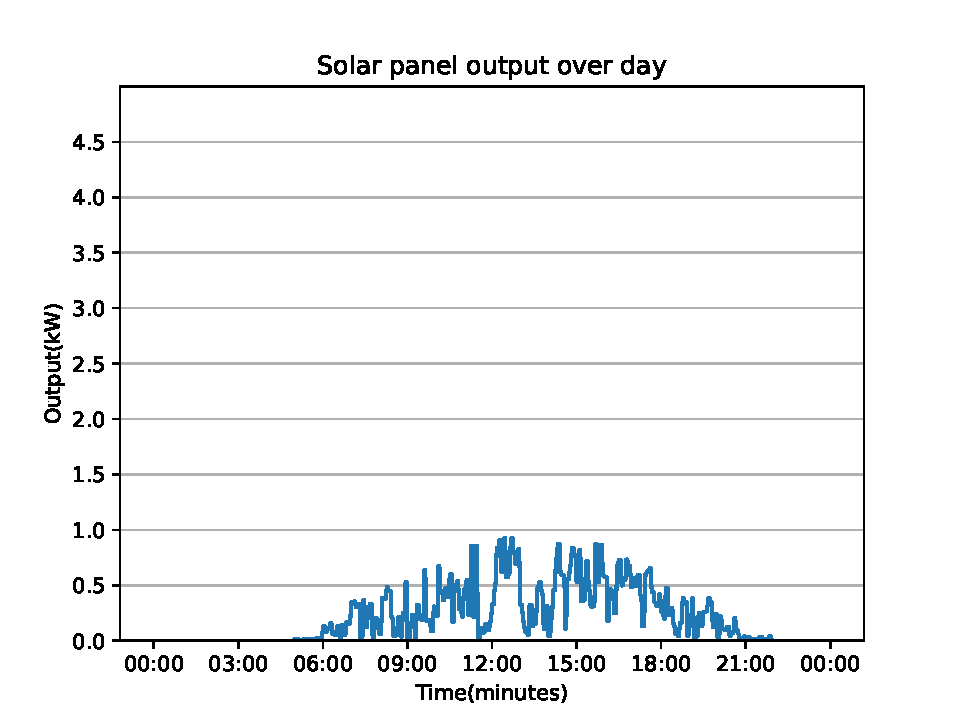
\includegraphics[width=\linewidth]{img/solar_day_cloudy.pdf}
\caption{Výkon solárního panelu během zataženého letního dne}
\label{fig:solar_day_cloudy}
\end{figure}

Ve výsledku elektrárna generuje výkon, jaký by se dal v dané oblasti - Brně očekávat \cite{Zilvar-2022}.

\begin{figure}
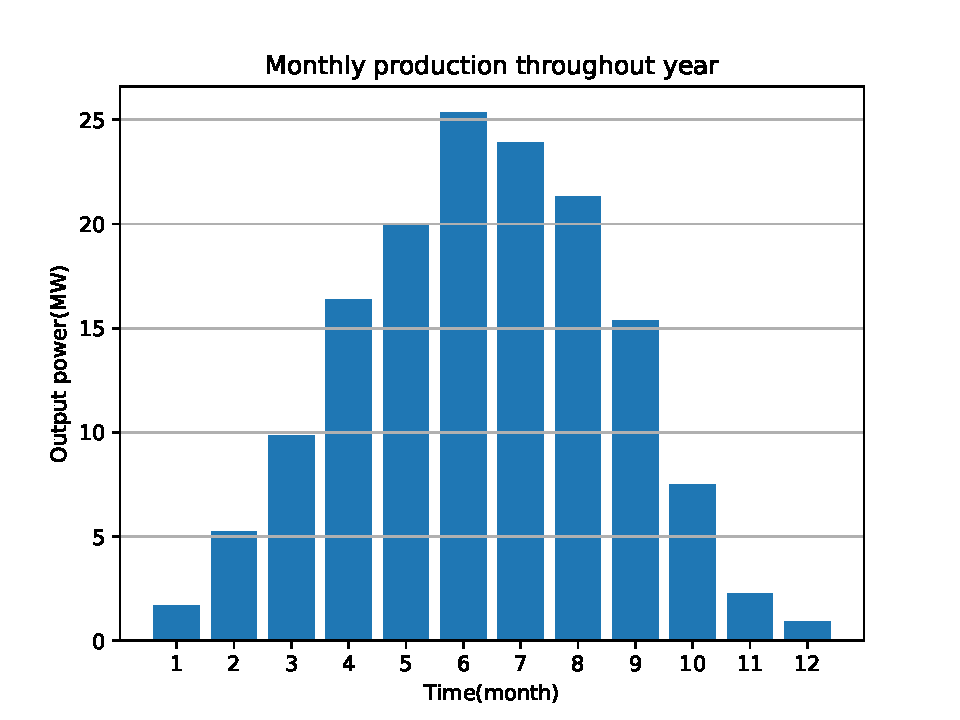
\includegraphics[width=\linewidth]{img/solar_power_hist.pdf}
\caption{Suma výkonů v jednotlivých měsících}
\label{fig:solar_power_hist}
\end{figure}

\subsection{Domácnost}
Modul domácnosti má za úkol náhodně modelovat spotřebu elektrické energie tak,
aby se co nejblíže podobal reálné domácnosti.
Má tedy jedinou výstupní proměnnou, která udává výkon spotřebovaný v daném čase.
Spotřeba domácnosti závisí na čase, ze kterého je spočítán den v týdnu a roční období.

Spotřeba v domácnosti je zcela nezávislá na výkonu elektrárny v daném čase.
Zde by mohl být drobný rozdíl oproti realitě.
Členové domácnosti mohou záměrně spotřebovávat více elektřiny, pokud má zrovna elektrárna přebytečný výkon.
Dobrý příklad tohoto by bylo zapnutí elektrické trouby, když je elektrárna v provozu.

\subsubsection{Implementace}
Domácnost je modelována jako proces knihovny SIMLIB.
Spotřeba je počítána jako součet konstantní a dynamické spotřeby.
Konstantní představuje výkon, který je odebírán vždy.
V reálné domácnosti by tento výkon představovaly například síťové modemy a switche.
Dále je do této části započítána pohotovostní spotřeba televizí, monitorů, počítačů a jiných spotřebičů.

Dynamická spotřeba představuje spotřebiče, které spotřebovávají energii pouze občas.
Toto je naprostá většina spotřebičů používaných v domácnosti.
Patřila by sem například varná konvice, elektrický sporák, televize, počítač a mnoho dalších.
Každý spotřebič má zadáno, mezi kterými časy se spouští a jaký podíl této doby je průměrně aktivní. [TODO mozna i neco dalsiho]
Podle těchto parametrů náhodně generuje zátěž.

Dynamická spotřeba je zcela nutná, aby byl model validní.
V případě, že by byla modelována pouze konstantní spotřeba,
celková spotřeba by mohla být stejná, ale spotřeba ze sítě resp. dodávka do sítě by se výrazně lišila.

Modul domácnosti periodicky sčítá výkon všech spotřebičů, který je monitorován monitorovacím zařízením.
Tato spotřeba je zobrazena na obrázku ~\ref{fig:load_power},
kde jedna křivka představuje okamžitou spotřebu a druhá šestihodinový pohyblivý průměr.

\begin{figure}
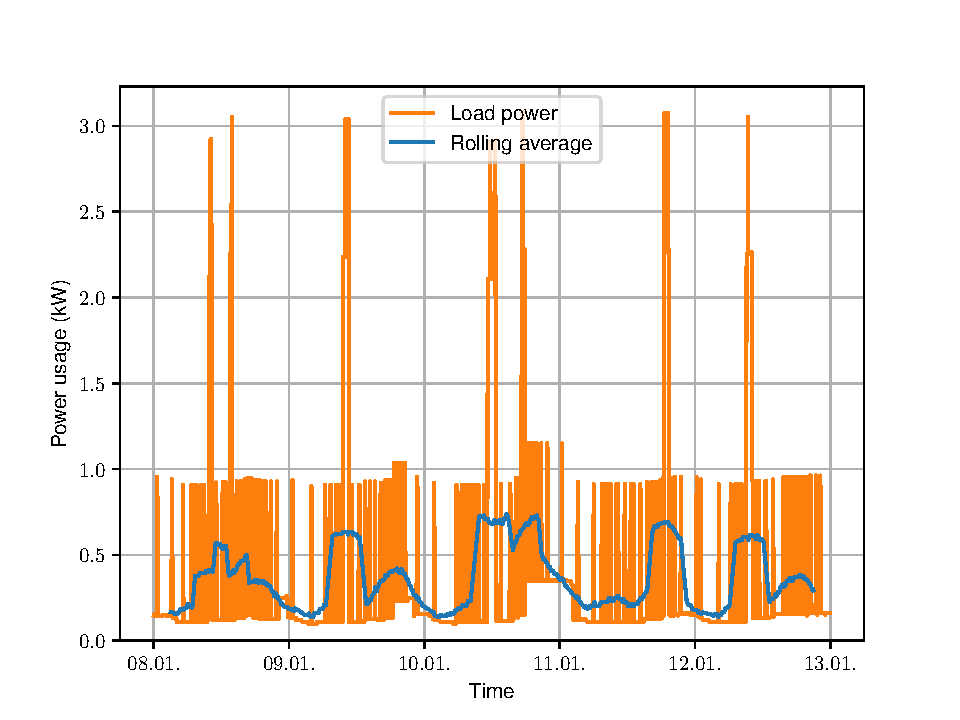
\includegraphics[width=\linewidth]{img/load_power.pdf}
\caption{Spotřeba domácnosti v rozsahu 5 dní}
\label{fig:load_power}
\end{figure}

\subsubsection{Spotřebiče}
Všechny spotřebiče jsou implementovány jako C++ objekty, přičemž jejich třídy vždy dědí ze třídy \texttt{Load}.
Rozhraní \texttt{Load} poskytuje metodu \texttt{readPower}, která vrací současný výkon spotřebiče.
Díky ní mohou být všechny odečítány modulem domácnosti.
Spotřebiče jsou implementovány třídami \texttt{Appliance} a \texttt{LightBulb}.

Spotřebiče třídy \texttt{Appliance} mají jako parametry výkon, průměrný čas běhu a pravděpodobnosti, že budou zapnuté pro každou hodinu.
Pravděpodobnosti jsou implementovány jako pole 24 položek typu float,
každá z nich určuje pravděpodobnost, že bude daný spotřebič v tu hodinu aktivní.
Konkrétní hodnoty byly převzaty ze studie \cite{Torriti-2017}.

Žárovky třídy \texttt{LightBulb} jsou implementovány tak,
že

\subsubsection{Verifikace modelu}

Pro ověření správné spotřeby v závislosti na čase byl sestrojen histogram,
který zobrazuje průměrnou spotřebu v každé hodině dne (Obrázek \ref{fig:average_day_load}).
Data jsou zprůměrována z 1 simulovaného roku roku.
Implementovaný model víceméně koresponduje s předlohou \cite{Torriti-2017}.

Celá domácnost spotřebuje 3.27 MWh za rok, což zhruba odpovídá průměrné spotřebě domácnosti v České Republice \cite{CEZ}.

\begin{figure}
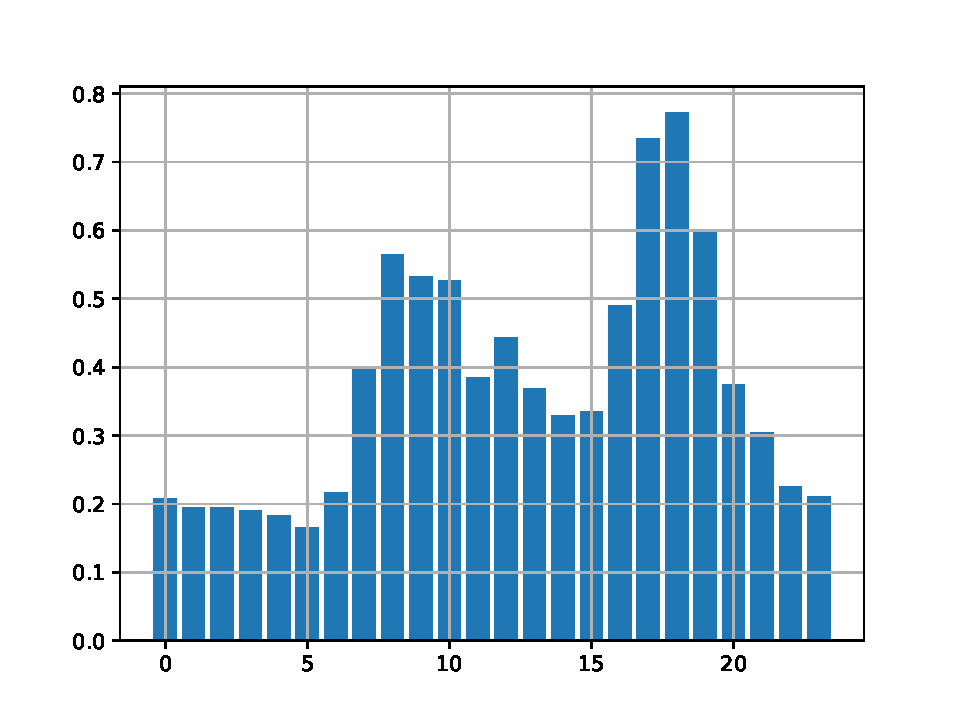
\includegraphics[width=\linewidth]{img/average_day_load.pdf}
\caption{Průměrná spotřeba domácnosti v každé hodině dne}
\label{fig:average_day_load}
\end{figure}

\subsection{Elektrické vozidlo}
Elektrické vozidlo je implementováno jako další proces knihovny SIMLIB.
V porovnání s realitou tento modul obsahuje více, než jen EV.
Obsahuje i nabíjecí stanici, která nabíjí vozidlo, případně dodává energii do sítě.
V tomto modulu jsou také počítány veškeré ztráty energie, ke kterým dochází při nabíjení, resp. vybíjení.

\subsubsection{Funkcionalita}
Tento modul může být nastaven na více režimů operace, a těmi jsou V2G, V1G, obyčejná nabíječka a žádné auto.
Režim V2G znamená, že EV se nabíjí podle toho, jestli je nějaký přebytek energie z elektrárny.
Dále v tomto režimu EV dodává elektřinu do sítě, pokud ho o to měřící zařízení požádá.
Může tak pokrýt spotřebu v domu, pokud zrovna elektrárna nedodává dostatený výkon.

V režimu V1G je zachováno nabíjení, které spotřebuje pouze přebytek energie v síti.
Oproti V2G ale EV nemůže dodávat energii do sítě.

V režimu obyčejné nabíječky EV nebere žádný ohled na současnou spotřebu v síti.
Nabíjí se konstantní rychlostí, dokud není baterie plná.

Modul také obsahuje režim, který představuje, že žádné EV není připojeno k síti.
Jedná se spíše o implementační detail, díky kterému lze simulaci provést i bez EV.

Maximální výkon pro nabíjení vozidla i dodávání energie zpět do sítě je 7,4 kW, podle TODO https://www.cleanenergyreviews.info/blog/bidirectional-ev-charging-v2g-v2h-v2l.

Dále má vozidlo nastavitelný režim provozu, podle kterého může vyjíždět z domu.
Implementovaný je režim, při kterém vozidlo jezdí do práce.
Vozidlo každý všední den po sedmé hodině vyjíždí a vrací se za 8 hodin.
V době, kdy je pryč mu také z baterie ubyde 5 kWh energie,
což odpovídá ujeté vzdálenosti 25 km. TODO zdroj https://ev-database.org/cheatsheet/energy-consumption-electric-car.

\subsubsection{Implementace}
Nabíjení vozidla a dodávání energie do sítě je implementováno metodami třídy v C++.
Objekt EV má proměnnou, ve které je současná energie, která je nabita v baterii.
Měřící nástroj může vozidlu poslat, že chce v následujícím měřícím úseku nabít do baterie nějaké množství energie.
Tato funkce vrátí skutečné množství energie, které bylo spotřebované vozidlem.
Pokud je množství energie za daný čas příliš velké,
vozidlo se nemůže nabíjet tak rychle, spotřebuje pouze množství omezené maximálním výkonem nabíječky.
Dodávka energie do sítě se řídí stejným pravidlem.

Pokud je EV na minimálním limitu baterie, nedodává již žádnou energii do sítě.
Pokud je naopak baterie plně nabitá, vozidlo nespotřebovává žádnou energii.



\subsection{Měřící zařízení}
Měřící zařízení je implementováno jako proces knihovny SIMLIB.
Tento proces provádí v pravidelných intervalech měření spořeby a výroby elektrické energie.
Pokud toto zařízení zjistí nadbytek energie v síti, dá EV možnost tuto energii spotřebovat.
Pokud je v síti naopak nedostatek energie a bylo by nutné ji brát od dodavatele, požádá EV o dodávku energie.
Poté spočítá sumu i s elekrickým vozidlem.
Všechny naměřené údaje jsou ukládány do sdíleného pole, aby šly přečíst a analyzovat po skončení simulace.

\section{Provedení simulace}

Simulace byla provedena vícekrát s různými prarametry.
Nastavitelnými parametry jsou režim vozidla (V2G, V1G, ...), kapacita baterie a provoz vozidla (jezdí do práce).

Jedna kombinace parametrů byla vybrána jeko bázový příklad,
oproti kterámu budou porovnávány ostatní.
Pro další případy je vždy změněn pouze jeden parametr.

\subsection{Základní příklad}

\bigskip
\begin{tabular}{ | c | c | c | }
\hline
Režim vozidla & Kapacita baterie & Provoz vozidla \\
\hline
V2G & 40 kWh & jezdí do práce \\
\hline
\end{tabular}
\bigskip

Pro bázový případ má vozidlo baterii o kapacitě 40 kWh, což je podle TODO zdroj průměr.
Vozidlo operuje v režimu V2G, protože ten je hlavním zaměřením studie.

\bigskip
\begin{tabular}{ | l | c | }
\hline
Energie odebraná od dodavatele & 2.480 MWh \\
\hline
Energie dodaná dodavateli & 2.332 MWh \\
\hline
Energie vyrobená solární elektrárnou & 4.992 MWh \\
\hline
Energie spotřebovaná domácností & 3.263 MWh \\
\hline
Energie nabitá do EV & 2.355 MWh \\
\hline
Energie obnovená z EV & 0.477 MWh \\
\hline
Energie spotřebovaná EV & 1.305 MWh \\
\hline
\end{tabular}
\bigskip


\subsection{V1G}

\bigskip
\begin{tabular}{ | c | c | c | }
\hline
Režim vozidla & Kapacita baterie & Provoz vozidla \\
\hline
V1G & 40 kWh & jezdí do práce \\
\hline
\end{tabular}
\bigskip

\bigskip
\begin{tabular}{ | l | c | }
\hline
Energie odebraná od dodavatele & 2.635 MWh \\
\hline
Energie dodaná dodavateli & 2.835 MWh \\
\hline
Energie vyrobená solární elektrárnou & 4.991 MWh \\
\hline
Energie spotřebovaná domácností & 3.263 MWh \\
\hline
Energie nabitá do EV & 1.529 MWh \\
\hline
Energie obnovená z EV & 0 MWh \\
\hline
Energie spotřebovaná EV & 1.305 MWh \\
\hline
\end{tabular}
\bigskip


\subsection{EV s běžnou nabíječkou}

\bigskip
\begin{tabular}{ | c | c | c | }
\hline
Režim vozidla & Kapacita baterie & Provoz vozidla \\
\hline
normální & 40 kWh & jezdí do práce \\
\hline
\end{tabular}
\bigskip

TODO napis vykon normalni nabijecky

\bigskip
\begin{tabular}{ | l | c | }
\hline
Energie odebraná od dodavatele & 3.183 MWh \\
\hline
Energie dodaná dodavateli & 3.354 MWh \\
\hline
Energie vyrobená solární elektrárnou & 4.992 MWh \\
\hline
Energie spotřebovaná domácností & 3.263 MWh \\
\hline
Energie nabitá do EV & 1.559 MWh \\
\hline
Energie obnovená z EV & 0 MWh \\
\hline
Energie spotřebovaná EV & 1.305 MWh \\
\hline
\end{tabular}
\bigskip


\subsection{Domácnost bez EV}

\bigskip
\begin{tabular}{ | c | c | c | }
\hline
Režim vozidla & Kapacita baterie & Provoz vozidla \\
\hline
neexistující & N/A & N/A \\
\hline
\end{tabular}
\bigskip

TODO spocitat, kolik by projelo benzinove auto.

\bigskip
\begin{tabular}{ | l | c | }
\hline
Energie odebraná od dodavatele & 2.133 MWh \\
\hline
Energie dodaná dodavateli &  3.862 MWh \\
\hline
Energie vyrobená solární elektrárnou & 4.992 MWh \\
\hline
Energie spotřebovaná domácností & 3.263 MWh \\
\hline
\end{tabular}
\bigskip


\subsection{EV s velkou baterií}

\bigskip
\begin{tabular}{ | c | c | c | }
\hline
Režim vozidla & Kapacita baterie & Provoz vozidla \\
\hline
V2G & 100 & jezdí do práce \\
\hline
\end{tabular}
\bigskip

V bázovém případě je uvažováno vozidlo s kapacitou baterie 40 kWh.
Na trhu ale existují auta s kapacitkou až 100 kWh.
Tento experiment je proveden pro porovnání rozdílů.

\bigskip
\begin{tabular}{ | l | c | }
\hline
Energie odebraná od dodavatele & 2.302 MWh \\
\hline
Energie dodaná dodavateli & 2.074 MWh \\
\hline
Energie vyrobená solární elektrárnou & 4.992 MWh \\
\hline
Energie spotřebovaná domácností & 3.263 MWh \\
\hline
Energie nabitá do EV & 2.547 MWh \\
\hline
Energie obnovená z EV & 0.588 MWh \\
\hline
Energie spotřebovaná EV & 1.305 MWh \\
\hline
\end{tabular}
\bigskip

Připojením auta s větší baterií bylo docíleno menší spořeby energie od dodavatele podle očekávání.
Rozdíl však není příliš velký při porovnání 2.480 MWh v bázovém případě a
2.302 MWh u auta s větší baterií.
Při běžné ceně energie tento rozdíl ušetří TODO za rok, což zřejmě nepokryje cenu auta s větší baterií.


\subsection{Trvale připojené vozidlo}

\bigskip
\begin{tabular}{ | c | c | c | }
\hline
Režim vozidla & Kapacita baterie & Provoz vozidla \\
\hline
V2G & 40 kWh & trvale připojeno \\
\hline
\end{tabular}
\bigskip

Ve všech ostatních případech je počítáno s tím, že je vozidlo využíváno pro dojíždění do práce.
Toto jsou často hodiny, kdy je elektrárna nejvíce aktivní.
Proto je proveden exprerimentm kdy je vozidlo připojeno trvale, nikdy neodjíždí.
Toto je sice velmi nerealistický případ, ale umožní zjistit vliv nepřítomnosti vozidla.

\bigskip
\begin{tabular}{ | l | c | }
\hline
Energie odebraná od dodavatele & 0.940 MWh \\
\hline
Energie dodaná dodavateli & 1.804 MWh \\
\hline
Energie vyrobená solární elektrárnou & 4.992 MWh \\
\hline
Energie spotřebovaná domácností & 3.263 MWh \\
\hline
Energie nabitá do EV & 2.058 MWh \\
\hline
Energie obnovená z EV & 1.193 MWh \\
\hline
Energie spotřebovaná EV & 0 MWh \\
\hline
\end{tabular}
\bigskip

Permanentně připojené vozidlo snížilo spotřebu od dodavatele podle očekávání.
Snížení z 2.480 MWh na 0.940 MWh je velmi výrazné.


\section{Závěr}

Provedená simulace dokázala, že ...

\printbibliography

\end{document}


















































